\section{Kantenerkennung}
\writtenby{\dcauthornameewie}%
Kanten in einem Bild zeigen sich durch abrupte Helligkeitsänderungen zwischen benachbarten Pixeln.
Um die Helligkeitsänderung für jedes Pixel zu bestimmen muss der Gradient der Helligkeitsfunktion $\nabla I$ eines Bildes berechnet werden.
Das gängigste Verfahren zur Bestimmung des Gradienten ist dessen Annäherung durch Faltung des Bildes $I$ mit einer Faltungsmatrix $K$ (auch genannt Kernel).
  \[ (I\circ K)(x,y) =
       \sum_{(u,v)\in m\times n}
       I\left(x+u-\frac{m}{2},y+v-\frac{n}{2}\right)K_{u,v}
       \quad K\in\mathbb{R}^{m\times n}
       \quad m,n \in\mathbb{N} \]
Die Berechnung eines einzelnen Gradientenbildes reicht jedoch nicht aus um alle Kanten eines Bildes zu erfassen, da die Faltungsmatrix nur Helligkeitsänderungen entlang einer Dimension erfasst.
Deshalb ist ein zweites Gradientenbild unter Verwendung einer Faltungsmatrix, die Helligkeitsänderungen entlang einer zweiten Dimension erfasst, erforderlich.
In der Regel nutzt man dafür die Transponierte der ersteren Faltungsmatrix.
Der Gradient der Helligkeitsfunktion ergibt sich  Berechnung 
  \[ \nabla I(x,y) = \sqrt{(I \circ K_X)(x,y)^2 + (I \circ K_Y)(x,y)^2} \]

\subsection*{Roberts-Operator}
Der \surname{Roberts}-Operator \cite{DBLP:books/garland/Roberts63} war eine der ersten Faltungsmatrizen die zur Kantenerkennung in technischen Strichzeichnungen verwendet wurde.
Im vergleich zu anderen Operatoren erzeugt er dünnere Kanten.
Hat dadurch aber den Vorteil Bildrauschen weniger stark als Kanten zu erfassen.
Da die Matrix $K_X$ identisch mit ihrer Transponierten ist vertauscht man die Spalten von $K_X$ um somit $K_Y$ zu erhalten.
  \[ K_X = \begin{vmatrix}
       1 &  0 \\
       0 & -1
     \end{vmatrix}
     \quad K_Y = \begin{vmatrix}
        0 & 1 \\
       -1 & 0
     \end{vmatrix} \]

\subsection*{Prewitt-Operator}
Der \surname{Prewitt}-Operator \cite[S.~108]{prewitt1070} erzeugt bereits dickere Kanten, und ist noch nicht so anfällig für Bildrauschen.
  \[ K_X = \begin{vmatrix}
       1 & 0 & -1 \\
       1 & 0 & -1 \\
       1 & 0 & -1
     \end{vmatrix}
     \quad K_Y = K_X^\top \]

\subsection*{Sobel-Operator}
Der \surname{Sobel}-Operator unterscheidet sich kaum vom \surname{Prewitt}-Operator.
Jedoch ist er bereits empfindlicher gegenüber Rauschen.
  \[ K_X = \begin{vmatrix}
       1 & 0 & -1 \\
       2 & 0 & -2 \\
       1 & 0 & -1
     \end{vmatrix}
     \quad K_Y = K_X^\top \]

\subsection*{Scharr-Operator}
Der \surname{Scharr}-Operator ist eine Weiterentwicklung des \surname{Sobel}-Operators mit besserer Rotationssymmetrie.
Erfasst Bildrauschen noch stärker als der \surname{Sobel}-Operator.
  \[ K_X = \begin{vmatrix}
        3 & 0 & -3 \\
       10 & 0 & -10 \\
        3 & 0 & -3
     \end{vmatrix}
     \quad K_Y = K_X^\top \]

\begin{figure}[H]
  \label{ref:edge-detection}
  \centering
  
\includegraphics[width=0.1925\textwidth]{img/basics/edge-detection/original}
  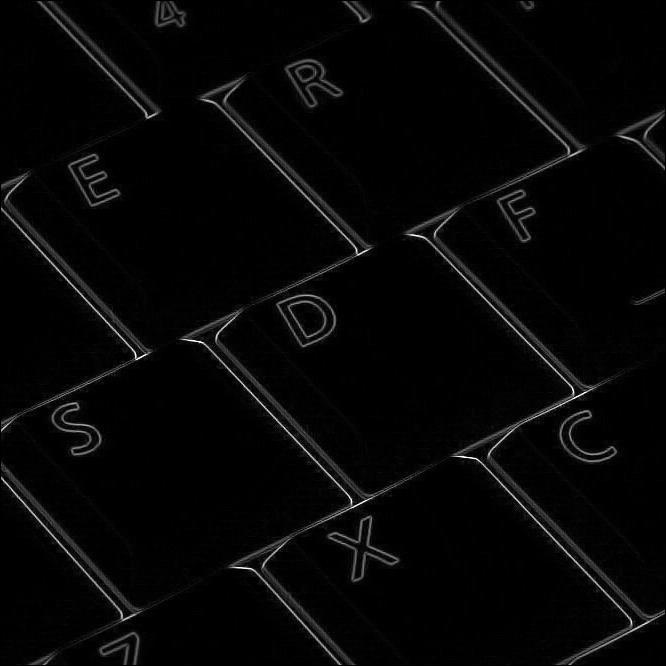
\includegraphics[width=0.1925\textwidth]{img/basics/edge-detection/roberts}
  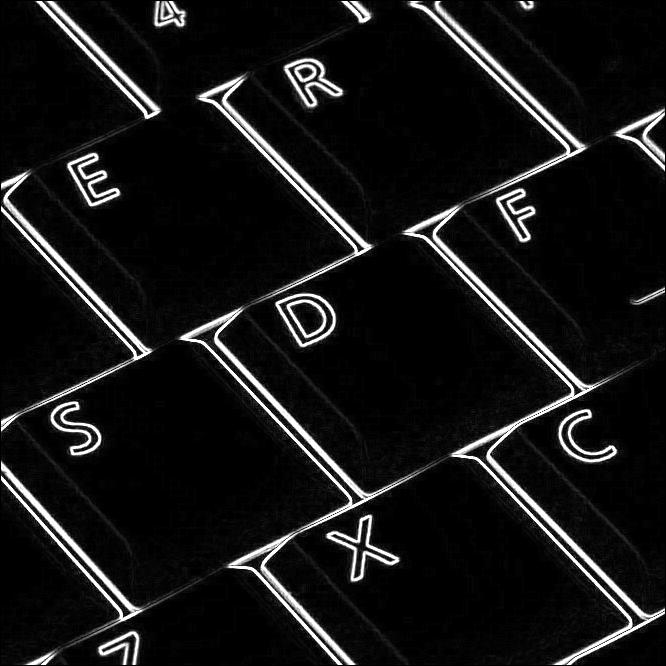
\includegraphics[width=0.1925\textwidth]{img/basics/edge-detection/prewitt}
  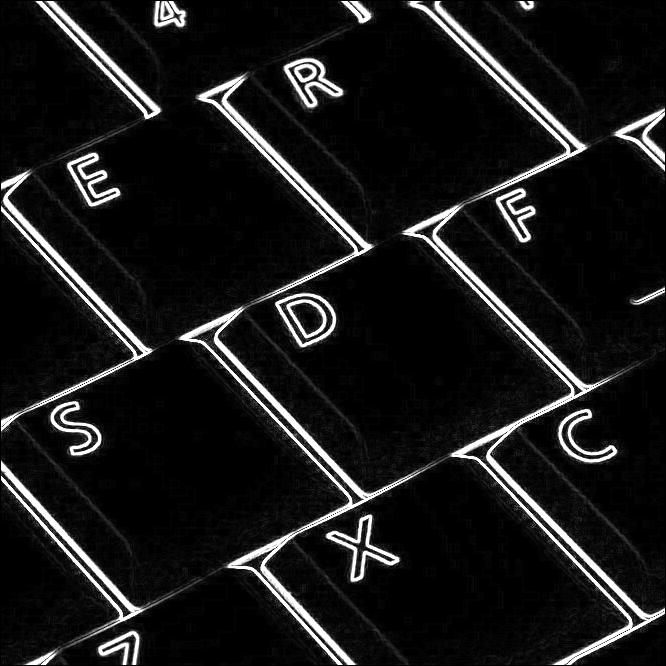
\includegraphics[width=0.1925\textwidth]{img/basics/edge-detection/sobel}
  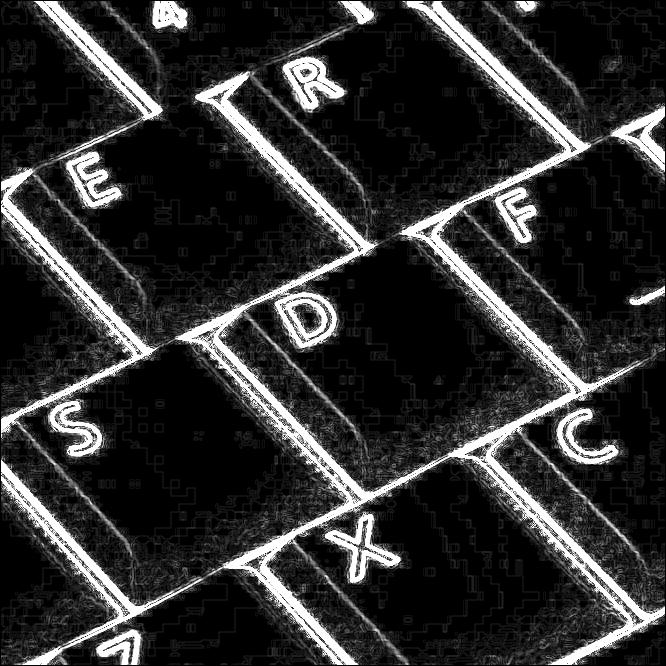
\includegraphics[width=0.1925\textwidth]{img/basics/edge-detection/scharr}
  \caption[Kantenerkennung]{Kantenerkennung eines Bildes\protect\footnotemark~(a) mit \surname{Roberts}-Operator (b), \surname{Prewitt}-Operator (c), \surname{Sobel}-Operator (d), und \surname{Scharr}-Operator (e) unter Verwendung der oben genannten Operatoren.}
\end{figure}

\footnotetext{\url{http://www.publicdomainpictures.net/view-image.php?image=1816}}
